\documentclass[12pt,a4paper]{article}

% ─── Page Layout ───────────────────────────────────────────────────────────────
\usepackage[a4paper, margin=0.8in, headheight=14pt]{geometry}

% ─── Fonts (XeLaTeX) ───────────────────────────────────────────────────────────
\usepackage{fontspec}
\usepackage{unicode-math}
\setmainfont{TeX Gyre Pagella}
\setmonofont[Scale=0.88]{TeX Gyre Cursor}
\setmathfont{Latin Modern Math}

% ─── Packages ──────────────────────────────────────────────────────────────────
\usepackage{xcolor}
\usepackage{colortbl}
\usepackage{titlesec}
\usepackage{enumitem}
\usepackage{tabularx}
\usepackage{booktabs}
\usepackage{array}
\usepackage{amsmath}
\usepackage{tikz}
\usetikzlibrary{shapes.geometric, arrows.meta, positioning, calc, fit, decorations.pathreplacing}
\usepackage{tcolorbox}
\tcbuselibrary{skins, breakable}
\usepackage{hyperref}
\usepackage{fancyhdr}
\usepackage{graphicx}
\usepackage{microtype}
\hyphenpenalty=10000
\exhyphenpenalty=10000
\sloppy
\usepackage{caption}
\usepackage{setspace}
\usepackage{multirow}
\usepackage{tocloft}

% ─── Q&A helper ────────────────────────────────────────────────────────────────
\newcommand{\Q}[1]{\textbf{#1}\par\noindent\ignorespaces}

% ─── Colour Palette ────────────────────────────────────────────────────────────
\definecolor{myred}{RGB}{196,30,58}
\definecolor{mydark}{RGB}{30,30,50}
\definecolor{mygreen}{RGB}{14,120,80}
\definecolor{myteal}{RGB}{0,130,140}
\definecolor{myamber}{RGB}{180,100,0}
\definecolor{mypurple}{RGB}{100,30,160}
\definecolor{mygray}{RGB}{246,247,249}
\definecolor{mgframe}{RGB}{180,185,200}
\definecolor{watermark}{RGB}{145,150,170}
\definecolor{hdrred}{RGB}{250,232,235}
\definecolor{hdrgreen}{RGB}{220,244,233}
\definecolor{hdrteal}{RGB}{220,242,244}
\definecolor{hdramber}{RGB}{253,242,215}
\definecolor{hdrpurple}{RGB}{238,228,255}
\definecolor{hdrgray}{RGB}{238,240,245}
\definecolor{rowalt}{RGB}{250,251,253}

% ─── Section Formatting ────────────────────────────────────────────────────────
\titleformat{\section}
  {\large\bfseries\color{myred}}{\thesection.}{0.5em}{}
  [\vspace{1pt}{\color{myred}\rule{\linewidth}{0.8pt}}]
\titleformat{\subsection}
  {\normalsize\bfseries\color{myteal}}{\thesubsection}{0.5em}{}
\titlespacing*{\section}{0pt}{18pt}{7pt}
\titlespacing*{\subsection}{0pt}{11pt}{4pt}

% ─── Paragraph ─────────────────────────────────────────────────────────────────
\setlength{\parindent}{0pt}
\setlength{\parskip}{4pt}

% ─── TOC Styling ───────────────────────────────────────────────────────────────
\renewcommand{\cfttoctitlefont}{\large\bfseries\color{myred}}
\renewcommand{\cftaftertoctitle}{\par\noindent{\color{myred}\rule{\linewidth}{0.8pt}}}
\setlength{\cftbeforetoctitleskip}{0pt}
\setlength{\cftaftertoctitleskip}{6pt}
\renewcommand{\cftsecfont}{\normalsize\bfseries\color{mydark}}
\renewcommand{\cftsecpagefont}{\normalsize\bfseries\color{mydark}}
\renewcommand{\cftsecleader}{\cftdotfill{\cftdotsep}}
\setlength{\cftbeforesecskip}{7pt}
\renewcommand{\cftsubsecfont}{\small\color{mydark}}
\renewcommand{\cftsubsecpagefont}{\small\color{mydark}}
\setlength{\cftbeforesubsecskip}{3pt}
\setlength{\cftsubsecindent}{1.4em}

% ─── Table helpers ─────────────────────────────────────────────────────────────
\renewcommand{\arraystretch}{1.45}
\setlength{\tabcolsep}{6pt}
\arrayrulecolor{mydark}
\newcolumntype{B}[1]{>{\small\bfseries\raggedright\arraybackslash}m{#1}}
\newcolumntype{Y}{>{\small\raggedright\arraybackslash}X}
\renewcommand{\tabularxcolumn}[1]{m{#1}}

% ─── Header / Footer ───────────────────────────────────────────────────────────
\pagestyle{fancy}
\fancyhf{}
\fancyhead[L]{\small\color{myred}\textbf{PE-EC603D}\;\color{mydark}--- Information Theory and Coding}
\fancyhead[R]{\small\color{myteal}\textbf{Module 3 Notes}}
\fancyfoot[C]{\small\color{mydark}\thepage}
\fancyfoot[R]{\small\color{watermark}\textit{\copyright\ Biraj}}
\renewcommand{\headrulewidth}{0.5pt}
\renewcommand{\footrulewidth}{0.3pt}

% ─── Hyperref ──────────────────────────────────────────────────────────────────
\hypersetup{
  colorlinks=true, linkcolor=myteal, urlcolor=myteal,
  pdfauthor={Biraj Sarkar},
  pdftitle={PE-EC603D --- Module 3 Notes}
}

% ─── tcolorbox styles ──────────────────────────────────────────────────────────
\tcbset{
  tikzbox/.style={
    colback=mygray, colframe=mgframe, boxrule=0.6pt, arc=4pt,
    left=8pt, right=8pt, top=6pt, bottom=6pt,
    colbacktitle=mgframe, coltitle=mydark,
    fonttitle=\small\bfseries
  },
  defbox/.style={
    colback=hdrgreen, colframe=mygreen, boxrule=0.8pt, arc=4pt,
    left=9pt, right=9pt, top=6pt, bottom=6pt,
    colbacktitle=mygreen, coltitle=white,
    fonttitle=\small\bfseries
  },
  formulabox/.style={
    colback=hdrteal, colframe=myteal, boxrule=0.8pt, arc=4pt,
    left=9pt, right=9pt, top=7pt, bottom=7pt,
    colbacktitle=myteal, coltitle=white,
    fonttitle=\small\bfseries
  },
  examplebox/.style={
    colback=hdramber, colframe=myamber, boxrule=0.8pt, arc=4pt,
    left=9pt, right=9pt, top=6pt, bottom=6pt,
    colbacktitle=myamber, coltitle=white,
    fonttitle=\small\bfseries
  },
  masonbox/.style={
    colback=hdrpurple, colframe=mypurple, boxrule=0.8pt, arc=4pt,
    left=9pt, right=9pt, top=6pt, bottom=6pt,
    colbacktitle=mypurple, coltitle=white,
    fonttitle=\small\bfseries
  },
  exambox/.style={
    colback=hdrpurple, colframe=mypurple, boxrule=1pt, arc=5pt,
    left=10pt, right=10pt, top=8pt, bottom=8pt,
    colbacktitle=mypurple, coltitle=white,
    fonttitle=\bfseries,
    breakable, title after break={\textbf{Frequently Asked / Viva Questions (contd.)}}}
}
% Make all boxes breakable across pages
\tcbset{breakable}

% ─── TikZ styles ───────────────────────────────────────────────────────────────
\tikzset{
  block/.style={rectangle, draw=myteal, fill=hdrteal,
    text width=2.4cm, align=center, minimum height=0.95cm,
    font=\small, rounded corners=3pt, line width=0.7pt},
  redblock/.style={rectangle, draw=myred, fill=hdrred,
    text width=2.4cm, align=center, minimum height=0.95cm,
    font=\small, rounded corners=3pt, line width=0.7pt},
  netnode/.style={rectangle, draw=myteal, fill=hdrteal,
    text width=1.5cm, align=center, minimum height=0.8cm,
    font=\small, rounded corners=3pt, line width=0.7pt},
  sumjunc/.style={circle, draw=myamber, fill=hdramber,
    minimum size=0.62cm, font=\small, line width=0.8pt},
  snode/.style={circle, draw=mypurple, fill=hdrpurple,
    minimum size=0.55cm, font=\footnotesize, line width=0.7pt},
  arrow/.style={-Stealth, thick, color=mydark},
  redarrow/.style={-Stealth, thick, color=myred},
  line/.style={thick, color=mydark}
}

% ═══════════════════════════════════════════════════════════════════════════════
\begin{document}
% ═══════════════════════════════════════════════════════════════════════════════

\begin{center}
  {\LARGE\bfseries\color{myred} PE-EC603D --- Information Theory and Coding}\\[5pt]
  {\normalsize\color{mydark} Semester VI \quad$\bullet$\quad 3L:0T:0P \quad$\bullet$\quad 3 Credits}\\[3pt]
  {\normalsize\color{myteal}\textbf{Module 3 Exam Notes: Coding Techniques \& Cyclic/Convolutional Codes}}\\[3pt]
  {\small\color{mydark} CGEC \;$|$\; B.Tech ECE (2023--27) \;$|$\; \textit{Biraj Sarkar}}
\end{center}
\vspace{2pt}
\noindent{\color{myred}\rule{\linewidth}{1.5pt}}
\vspace{2pt}

\hypersetup{linkcolor=mydark}
\tableofcontents
\hypersetup{linkcolor=myteal}
\newpage

% ===============================================================================
\section{Huffman Coding}
% ===============================================================================

Huffman coding is an optimal source coding technique used for lossy/lossless data compression. It belongs to the class of prefix-free codes, which are uniquely detectable.

\subsection{Definition and Concept}
\begin{tcolorbox}[defbox]
\textbf{Huffman Coding:} A bottom-up, variable-length source coding algorithm that assigns binary codes to symbols based on their probabilities. High-probability symbols are assigned shorter codewords, and low-probability symbols are assigned longer codewords, minimizing average codeword length.
\end{tcolorbox}

\subsection{The Huffman Coding Algorithm}
\begin{enumerate}[label=\textbf{Step \arabic*:}, leftmargin=4.5em, itemsep=3.5pt]
  \item Sort the source symbols in descending order of their probabilities.
  \item Combine the two lowest-probability symbols into a single node (parent node) with a probability equal to the sum of their probabilities.
  \item Assign binary '0' to one branch of the pair (usually the upper/higher probability branch) and '1' to the other branch.
  \item Place the combined node back into the list and re-sort all items in descending order.
  \item Repeat Steps 2 to 4 recursively until only one root node (probability = 1.0) remains.
  \item The codeword for each symbol is read by tracing the path from the root of the tree down to the symbol leaf node.
\end{enumerate}

\begin{tcolorbox}[examplebox, title={Worked Example: Huffman Coding}]
\textbf{Problem:} A discrete source emits 5 symbols $\{s_1, s_2, s_3, s_4, s_5\}$ with probabilities $P = \{0.4, 0.2, 0.2, 0.1, 0.1\}$.
\begin{enumerate}[label=\alph*., leftmargin=*, itemsep=1pt, topsep=1pt]
  \item Construct the Huffman code tree and determine the codewords.
  \item Calculate the average codeword length $L$ and coding efficiency $\eta$.
\end{enumerate}
\textbf{Solution:}

\textbf{(a) Tree Construction and Codewords:}
Tracing from the lowest probabilities up (bottom-up merging):
\begin{itemize}[leftmargin=*, itemsep=1pt]
  \item Merge $s_4$ (0.1) and $s_5$ (0.1) to create node $N_1$ with probability $0.2$. Assign 0 to $s_4$ and 1 to $s_5$.
  \item We now have nodes with probabilities $\{0.4, 0.2, 0.2, 0.2\}$. Merge the two lowest, say $s_3$ (0.2) and $N_1$ (0.2) to create $N_2$ with probability $0.4$. Assign 0 to $s_3$ and 1 to $N_1$.
  \item We now have $\{0.4, 0.4, 0.2\}$. Merge $s_2$ (0.2) and $N_2$ (0.4) to create $N_3$ with probability $0.6$. Assign 0 to $s_2$ and 1 to $N_2$.
  \item Merge $s_1$ (0.4) and $N_3$ (0.6) to create the root (1.0). Assign 0 to $s_1$ and 1 to $N_3$.
\end{itemize}

\begin{tabularx}{\linewidth}{|B{1.6cm}|Y|Y|B{1.8cm}|}
\hline
\textbf{Symbol} & \textbf{Probability ($P_i$)} & \textbf{Codeword Path} & \textbf{Length ($l_i$)} \\
\hline
$s_1$ & 0.4 & 0 & 1 \\
$s_2$ & 0.2 & 10 & 2 \\
$s_3$ & 0.2 & 110 & 3 \\
$s_4$ & 0.1 & 1110 & 4 \\
$s_5$ & 0.1 & 1111 & 4 \\
\hline
\end{tabularx}

\textbf{(b) Calculations:}
Source Entropy $H(X)$:
\begin{align*}
  H(X) &= -[0.4\log_2 0.4 + 2 \times (0.2\log_2 0.2) + 2 \times (0.1\log_2 0.1)] \\
  &= -[0.4(-1.3219) + 0.4(-2.3219) + 0.2(-3.3219)] \\
  &= -[-0.5288 - 0.9288 - 0.6644] = 2.122 \text{ bits/symbol}
\end{align*}
Average Codeword Length $L$:
\begin{align*}
  L &= \sum P_i l_i = (0.4 \times 1) + (0.2 \times 2) + (0.2 \times 3) + (0.1 \times 4) + (0.1 \times 4) \\
  &= 0.4 + 0.4 + 0.6 + 0.4 + 0.4 = 2.2 \text{ bits/symbol} \\[4pt]
  \text{Efficiency } \eta &= \frac{H(X)}{L} = \frac{2.122}{2.2} \times 100\% = 96.45\%
\end{align*}
\end{tcolorbox}

\begin{tcolorbox}[tikzbox, title={Huffman Coding Tree Diagram}]
\centering
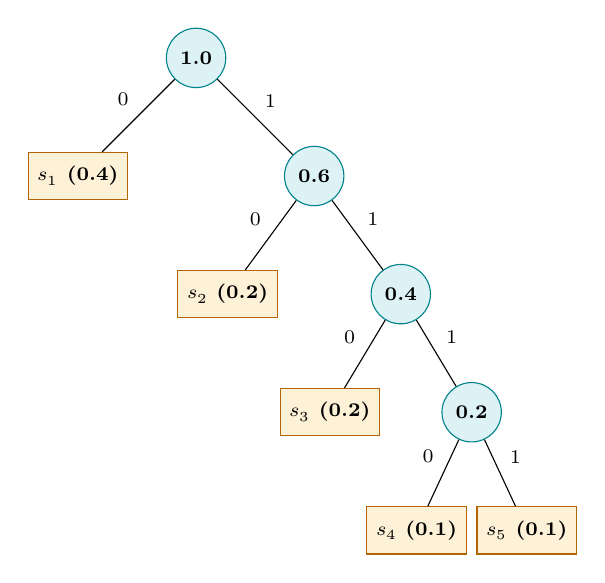
\begin{tikzpicture}[level distance=1.5cm,
  level 1/.style={sibling distance=3.0cm},
  level 2/.style={sibling distance=2.2cm},
  level 3/.style={sibling distance=1.8cm},
  level 4/.style={sibling distance=1.4cm},
  tnode/.style={circle, draw=myteal, fill=hdrteal, minimum size=0.6cm, font=\scriptsize\bfseries},
  leaf/.style={rectangle, draw=myamber, fill=hdramber, minimum size=0.6cm, font=\scriptsize\bfseries}]

  \node[tnode] (root) {1.0}
    child {node[leaf] (s1) {$s_1$ (0.4)}
      edge from parent node[above left, font=\scriptsize] {0}
    }
    child {node[tnode] (n3) {0.6}
      child {node[leaf] (s2) {$s_2$ (0.2)}
        edge from parent node[above left, font=\scriptsize] {0}
      }
      child {node[tnode] (n2) {0.4}
        child {node[leaf] (s3) {$s_3$ (0.2)}
          edge from parent node[above left, font=\scriptsize] {0}
        }
        child {node[tnode] (n1) {0.2}
          child {node[leaf] (s4) {$s_4$ (0.1)}
            edge from parent node[above left, font=\scriptsize] {0}
          }
          child {node[leaf] (s5) {$s_5$ (0.1)}
            edge from parent node[above right, font=\scriptsize] {1}
          }
          edge from parent node[above right, font=\scriptsize] {1}
        }
        edge from parent node[above right, font=\scriptsize] {1}
      }
      edge from parent node[above right, font=\scriptsize] {1}
    };
\end{tikzpicture}
\end{tcolorbox}

% ===============================================================================
\section{Cyclic Codes}
% ===============================================================================

Channel coding techniques inject structured redundancy into data packets to allow detection and correction of channel-induced errors.

\subsection{Definition of Cyclic Codes}
\begin{tcolorbox}[defbox]
\textbf{Cyclic Code:} A linear block code $(n, k)$ with the algebraic property that any cyclic shift of a valid codeword is also a valid codeword.
\par\vspace{3pt}
If $C = (c_0, c_1, \dots, c_{n-1})$ is a codeword, then $C^{(1)} = (c_{n-1}, c_0, \dots, c_{n-2})$ is also a codeword.
\end{tcolorbox}

In polynomial representation, a codeword is represented as:
\begin{equation}
  c(x) = c_0 + c_1 x + c_2 x^2 + \dots + c_{n-1} x^{n-1}
\end{equation}
The cyclic shift property means that if $c(x)$ is a codeword, then the remainder of $x c(x)$ divided by $x^n + 1$ is also a codeword.

\subsection{Generator Polynomial $g(x)$}
Every cyclic code is uniquely defined by a **generator polynomial** $g(x)$ of degree $n-k$.
\begin{itemize}[leftmargin=*, itemsep=2pt]
  \item $g(x)$ must be a factor of the polynomial $x^n + 1$ over GF(2) (Galois Field of 2, modulo-2 arithmetic).
  \item A polynomial $c(x)$ of degree $\le n-1$ is a valid codeword if and only if it is a multiple of $g(x)$:
    \begin{equation}
      c(x) = m(x) \cdot g(x)
    \end{equation}
    Where $m(x)$ is the message polynomial of degree $\le k-1$.
\end{itemize}

\subsection{Systematic Encoding of Cyclic Codes}
In systematic codes, the first $k$ bits represent the message directly, and the remaining $n-k$ bits are parity check bits.
\begin{tcolorbox}[formulabox, title={\textbf{Systematic Cyclic Coding Steps}}]
For message polynomial $m(x)$ and generator polynomial $g(x)$ of degree $n-k$:
\begin{enumerate}[label=\textbf{Step \arabic*:}, leftmargin=4.5em, itemsep=2pt, topsep=1pt]
  \item Multiply the message polynomial by $x^{n-k}$:
    \begin{equation*}
      u(x) = x^{n-k} m(x)
    \end{equation*}
  \item Divide $u(x)$ by $g(x)$ to obtain the remainder polynomial $r(x)$:
    \begin{equation*}
      \frac{x^{n-k} m(x)}{g(x)} = q(x) + \frac{r(x)}{g(x)} \implies r(x) = \text{rem}\left[ \frac{x^{n-k} m(x)}{g(x)} \right]
    \end{equation*}
  \item Form the codeword polynomial $c(x)$ by adding the remainder $r(x)$ to $u(x)$ (addition is XOR in GF(2)):
    \begin{equation}
      c(x) = x^{n-k} m(x) + r(x)
    \end{equation}
\end{enumerate}
\end{tcolorbox}

\begin{tcolorbox}[examplebox, title={Worked Example: (7, 4) Cyclic Systematic Code}]
\textbf{Problem:} For a $(7, 4)$ cyclic code, the generator polynomial is $g(x) = x^3 + x + 1$. Encode the message vector $m = [1, 0, 1, 1]$ systematically.\\[4pt]
\textbf{Solution:}
Identify parameters: $n=7$, $k=4$, $n-k=3$.
Convert message vector to polynomial:
\begin{equation*}
  m(x) = 1 \cdot x^0 + 0 \cdot x^1 + 1 \cdot x^2 + 1 \cdot x^3 = 1 + x^2 + x^3
\end{equation*}
Multiply $m(x)$ by $x^{n-k} = x^3$:
\begin{equation*}
  x^3 m(x) = x^3 (1 + x^2 + x^3) = x^3 + x^5 + x^6
\end{equation*}
Divide $x^3 m(x)$ by $g(x) = x^3 + x + 1$ using modulo-2 long division:
\begin{align*}
  &\text{Divide: } x^6 + x^5 + x^3 \text{ by } x^3 + x + 1 \\
  &x^6 + x^5 + x^3 = x^3(x^3 + x + 1) + x^5 + x^4 \quad (\text{since } x^6+x^4+x^3 \text{ subtracted leaves } x^5+x^4) \\
  &\text{Continuing long division gives: } \\
  &x^3 + x + 1 \overline{) x^6 + x^5 + 0x^4 + x^3} \\
  &\phantom{x^3 + x + 1} \underline{x^6 + 0x^5 + x^4 + x^3} \quad (\text{multiply by } x^3) \\
  &\phantom{x^3 + x + 1} \phantom{x^6 + } x^5 + x^4 + 0x^3 \\
  &\phantom{x^3 + x + 1} \phantom{x^6 + } \underline{x^5 + 0x^4 + x^3 + x^2} \quad (\text{multiply by } x^2) \\
  &\phantom{x^3 + x + 1} \phantom{x^6 + x^5 + } x^4 + x^3 + x^2 \\
  &\phantom{x^3 + x + 1} \phantom{x^6 + x^5 + } \underline{x^4 + 0x^3 + x^2 + x} \quad (\text{multiply by } x) \\
  &\phantom{x^3 + x + 1} \phantom{x^6 + x^5 + x^4 + } x^3 + 0x^2 + x \\
  &\phantom{x^3 + x + 1} \phantom{x^6 + x^5 + x^4 + } \underline{x^3 + 0x^2 + x + 1} \quad (\text{multiply by } 1) \\
  &\phantom{x^3 + x + 1} \phantom{x^6 + x^5 + x^4 + x^3 + } 1 \quad (\text{Remainder})
\end{align*}
Thus, the remainder is $r(x) = 1$.
Construct the codeword:
\begin{align*}
  c(x) &= x^3 m(x) + r(x) = (x^6 + x^5 + x^3) + 1 = 1 + x^3 + x^5 + x^6
\end{align*}
Convert polynomial to codeword vector:
\begin{equation*}
  C = [1, 0, 0, 1, 0, 1, 1]
\end{equation*}
Where the first 3 bits $[1, 0, 0]$ represent the parity check bits, and the last 4 bits $[1, 0, 1, 1]$ represent the message.
\end{tcolorbox}

\subsection{Hardware Encoder using Feedback Shift Registers (FSR)}
Cyclic codes are popular because their encoding and syndrome circuits can be implemented efficiently in hardware using shift registers and XOR gates (modulo-2 adders).

\begin{tcolorbox}[tikzbox, title={Feedback Shift Register Encoder for $g(x) = x^3 + x + 1$}]
\centering
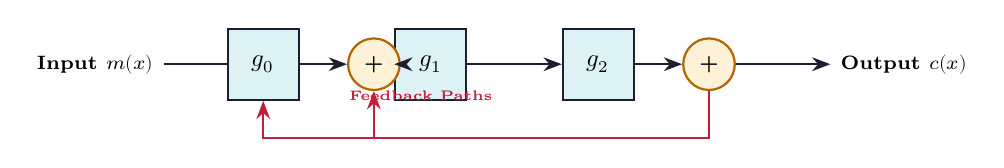
\begin{tikzpicture}[node distance=1.2cm, thick]
  % Draw registers
  \node[rectangle, draw=mydark, fill=hdrteal, minimum size=0.9cm, font=\small\bfseries] (R0) {$g_0$};
  \node[rectangle, draw=mydark, fill=hdrteal, minimum size=0.9cm, right=1.2cm of R0, font=\small\bfseries] (R1) {$g_1$};
  \node[rectangle, draw=mydark, fill=hdrteal, minimum size=0.9cm, right=1.2cm of R1, font=\small\bfseries] (R2) {$g_2$};

  % XOR sum junction (modulo 2 addition)
  \node[circle, draw=myamber, fill=hdramber, minimum size=0.5cm, right=0.6cm of R0, font=\scriptsize\bfseries] (xor1) {+};
  \node[circle, draw=myamber, fill=hdramber, minimum size=0.5cm, right=0.6cm of R2, font=\scriptsize\bfseries] (xor2) {+};

  % Input & Output
  \node (in) [left=0.8cm of R0, font=\scriptsize\bfseries] {Input $m(x)$};
  \node (out) [right=1.2cm of xor2, font=\scriptsize\bfseries] {Output $c(x)$};

  % Inter-register wires
  \draw[arrow] (R0) -- (xor1);
  \draw[arrow] (xor1) -- (R1);
  \draw[arrow] (R1) -- (R2);
  \draw[arrow] (R2) -- (xor2);
  \draw[arrow] (xor2) -- (out);

  % Feedback paths
  \draw[line] (in) -- (R0);
  \draw[redarrow] (xor2.south) -- ++(0,-0.6) -| (xor1.south);
  \draw[redarrow] (xor2.south) -- ++(0,-0.6) -| (R0.south);
  
  \node[font=\tiny\bfseries\color{myred}] at (2.0, -0.4) {Feedback Paths};
\end{tikzpicture}
\end{tcolorbox}

% ===============================================================================
\section{Convolutional Codes}
% ===============================================================================

Linear block codes processes data block-by-block. **Convolutional codes**, in contrast, process information continuously, using internal shift-register states to create memory dependencies.

\subsection{Basic Principles and Structure}
A convolutional encoder is defined by three parameters $(n, k, K)$:
\begin{itemize}[leftmargin=*, itemsep=2pt]
  \item $n$: Number of output bits produced in each shift cycle.
  \item $k$: Number of input bits processed in each shift cycle.
  \item $K$: Constraint length (number of shift register stages that affect the output).
\end{itemize}
The code rate is defined as $r = k/n$. The outputs are computed by modulo-2 addition of the current input and the values stored in the shift registers.

\begin{tcolorbox}[tikzbox, title={Convolutional Encoder Circuit (Rate $1/2$, Constraint Length $K=3$)}]
\centering
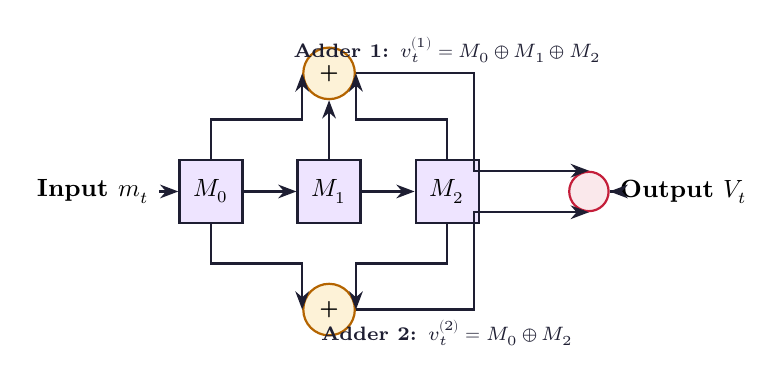
\begin{tikzpicture}[node distance=1.0cm, thick]
  % Input
  \node (in) at (-1.5, 0) [font=\small\bfseries] {Input $m_t$};

  % Shift Registers
  \node[rectangle, draw=mydark, fill=hdrpurple, minimum width=0.8cm, minimum height=0.8cm, font=\small\bfseries] (S0) at (0, 0) {$M_0$};
  \node[rectangle, draw=mydark, fill=hdrpurple, minimum width=0.8cm, minimum height=0.8cm, font=\small\bfseries] (S1) at (1.5, 0) {$M_1$};
  \node[rectangle, draw=mydark, fill=hdrpurple, minimum width=0.8cm, minimum height=0.8cm, font=\small\bfseries] (S2) at (3.0, 0) {$M_2$};

  % Modulo-2 adders (XOR)
  \node[circle, draw=myamber, fill=hdramber, minimum size=0.55cm, font=\scriptsize\bfseries] (xor1) at (1.5, 1.5) {+};
  \node[circle, draw=myamber, fill=hdramber, minimum size=0.55cm, font=\scriptsize\bfseries] (xor2) at (1.5, -1.5) {+};

  % Output selector switch
  \node[circle, draw=myred, fill=hdrred, minimum size=0.5cm] (sw) at (4.8, 0) {};
  \node (out) at (6.0, 0) [font=\small\bfseries] {Output $V_t$};

  % Connections
  \draw[arrow] (in) -- (S0);
  \draw[arrow] (S0) -- (S1);
  \draw[arrow] (S1) -- (S2);

  % Wires to XOR 1 (Upper Adder)
  \draw[arrow] (S0.north) -- ++(0,0.5) -| (xor1.west);
  \draw[arrow] (S1.north) -- (xor1.south);
  \draw[arrow] (S2.north) -- ++(0,0.5) -| (xor1.east);

  % Wires to XOR 2 (Lower Adder)
  \draw[arrow] (S0.south) -- ++(0,-0.5) -| (xor2.west);
  \draw[arrow] (S2.south) -- ++(0,-0.5) -| (xor2.east);

  % Output switch routing
  \draw[arrow] (xor1.east) -- ++(1.5,0) |- (sw.north);
  \draw[arrow] (xor2.east) -- ++(1.5,0) |- (sw.south);
  \draw[arrow] (sw) -- (out);

  % Labels
  \node[font=\scriptsize\bfseries\color{mydark}] at (3.0, 1.8) {Adder 1: $v^{(1)}_t = M_0 \oplus M_1 \oplus M_2$};
  \node[font=\scriptsize\bfseries\color{mydark}] at (3.0, -1.8) {Adder 2: $v^{(2)}_t = M_0 \oplus M_2$};
\end{tikzpicture}
\end{tcolorbox}

\subsection{Representations of Convolutional Codes}
Three graphical methods are used to describe a convolutional code:
\begin{enumerate}[label=\textbf{\arabic*.}, leftmargin=*, itemsep=3pt]
  \item \textbf{State Diagram:} Shows the states of the shift registers (excluding the current input) and the transitions between states caused by input '0' or '1'.
  \item \textbf{Tree Diagram:} Shows all possible output paths as a branching tree structure, where the path branches upward for input '0' and downward for input '1'.
  \item \textbf{Trellis Diagram:} A time-extended state transition diagram. It lists all possible states vertically at each time step, and shows transitions horizontally.
\end{enumerate}

\begin{tcolorbox}[tikzbox, title={Trellis Diagram Transition Segment}]
\centering
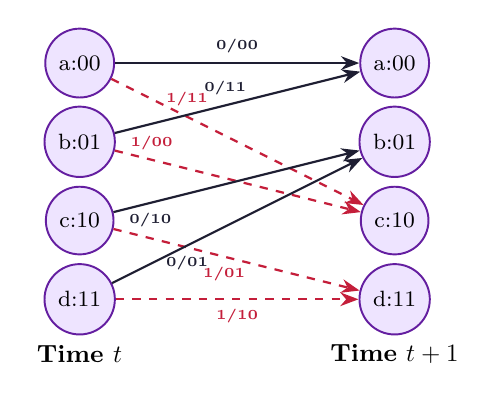
\begin{tikzpicture}[node distance=1.5cm, thick]
  % Define states at time t
  \node[snode] (a_t) at (0, 3) {a:00};
  \node[snode] (b_t) at (0, 2) {b:01};
  \node[snode] (c_t) at (0, 1) {c:10};
  \node[snode] (d_t) at (0, 0) {d:11};

  % Define states at time t+1
  \node[snode] (a_t1) at (4, 3) {a:00};
  \node[snode] (b_t1) at (4, 2) {b:01};
  \node[snode] (c_t1) at (4, 1) {c:10};
  \node[snode] (d_t1) at (4, 0) {d:11};

  % Transitions from state 'a' (input 0 -> solid; input 1 -> dashed)
  \draw[arrow] (a_t) -- (a_t1) node[midway, above, font=\tiny\bfseries] {0/00};
  \draw[arrow, dashed, color=myred] (a_t) -- (c_t1) node[pos=0.3, above, font=\tiny\bfseries\color{myred}] {1/11};

  % Transitions from state 'b'
  \draw[arrow] (b_t) -- (a_t1) node[pos=0.45, above, font=\tiny\bfseries] {0/11};
  \draw[arrow, dashed, color=myred] (b_t) -- (c_t1) node[pos=0.15, above, font=\tiny\bfseries\color{myred}] {1/00};

  % Transitions from state 'c'
  \draw[arrow] (c_t) -- (b_t1) node[pos=0.15, below, font=\tiny\bfseries] {0/10};
  \draw[arrow, dashed, color=myred] (c_t) -- (d_t1) node[pos=0.45, below, font=\tiny\bfseries\color{myred}] {1/01};

  % Transitions from state 'd'
  \draw[arrow] (d_t) -- (b_t1) node[pos=0.3, below, font=\tiny\bfseries] {0/01};
  \draw[arrow, dashed, color=myred] (d_t) -- (d_t1) node[midway, below, font=\tiny\bfseries\color{myred}] {1/10};

  % Time step indicators
  \node at (0, -0.7) [font=\small\bfseries] {Time $t$};
  \node at (4, -0.7) [font=\small\bfseries] {Time $t+1$};
\end{tikzpicture}
\end{tcolorbox}

\subsection{Viterbi Decoding Algorithm}
The Viterbi algorithm is the standard decoding method for convolutional codes. It finds the most likely sequence of transmitted symbols (minimum Hamming distance path) through the trellis.
\begin{itemize}[leftmargin=*, itemsep=3.5pt]
  \item \textbf{Branch Metric:} The Hamming distance between the received bits and the expected output bits for a specific branch.
  \item \textbf{Path Metric:} The accumulated sum of branch metrics along a path.
  \item \textbf{Survivor Path:} At each node in the trellis, the incoming path with the lowest path metric is saved, and all other paths are discarded. This prevents exponential path growth.
\end{itemize}

% ===============================================================================
\section{Arithmetic Coding}
% ===============================================================================

Huffman coding assigns an integer number of bits to each symbol. If a symbol has a probability of $0.9$, its ideal code length is $-\log_2 0.9 \approx 0.15$ bits, but Huffman must assign at least 1 bit, reducing efficiency. **Arithmetic coding** overcomes this constraint.

\subsection{Core Concept}
\begin{tcolorbox}[defbox]
\textbf{Arithmetic Coding:} A non-block source coding algorithm that maps an entire sequence of symbols to a single fractional number in the interval $[0, 1)$. Symbols are represented by ranges proportional to their probabilities.
\end{tcolorbox}

\subsection{Encoding Procedure}
\begin{enumerate}[label=\textbf{Step \arabic*:}, leftmargin=4.5em, itemsep=2pt, topsep=1pt]
  \item Initialize the interval boundaries: $\text{Low} = 0$, $\text{High} = 1$.
  \item For each symbol in the message:
    \begin{align}
      \text{Range} &= \text{High} - \text{Low} \\
      \text{High} &= \text{Low} + \text{Range} \times \text{Upper\_Cum\_Prob}(s_i) \\
      \text{Low} &= \text{Low} + \text{Range} \times \text{Lower\_Cum\_Prob}(s_i)
    \end{align}
  \item Repeat for all symbols in the sequence.
  \item The final output is any floating-point number within the final $[\text{Low}, \text{High})$ interval.
\end{enumerate}

\begin{tcolorbox}[examplebox, title={Worked Example: Arithmetic Coding of "WET"}]
\textbf{Problem:} A source has three symbols $\{E, T, W\}$ with probabilities $\{0.5, 0.3, 0.2\}$.
\begin{enumerate}[label=\alph*., leftmargin=*, itemsep=1pt, topsep=1pt]
  \item Calculate the cumulative probability ranges for the symbols.
  \item Encode the sequence "WET".
\end{enumerate}
\textbf{Solution:}

\textbf{(a) Probability Ranges:}\par\noindent
Sort alphabet (say alphabetically $\{E, T, W\}$):
\begin{itemize}[leftmargin=*, itemsep=1pt]
  \item Symbol $E$ (prob = 0.5): Cumulative Interval $[0.0, 0.5)$
  \item Symbol $T$ (prob = 0.3): Cumulative Interval $[0.5, 0.8)$
  \item Symbol $W$ (prob = 0.2): Cumulative Interval $[0.8, 1.0)$
\end{itemize}

\textbf{(b) Encode "WET":}
\begin{itemize}[leftmargin=*, itemsep=3pt]
  \item \textbf{Initial State:} $\text{Low} = 0$, $\text{High} = 1$, $\text{Range} = 1.0$.
  \item \textbf{First Symbol: 'W'} (Sub-interval $[0.8, 1.0)$):
    \begin{align*}
      \text{Low} &= 0 + 1.0 \times 0.8 = 0.8 \\
      \text{High} &= 0 + 1.0 \times 1.0 = 1.0 \\
      \text{Range} &= 1.0 - 0.8 = 0.2
    \end{align*}
  \item \textbf{Second Symbol: 'E'} (Sub-interval $[0.0, 0.5)$ relative to current range):
    \begin{align*}
      \text{Low} &= 0.8 + 0.2 \times 0.0 = 0.8 \\
      \text{High} &= 0.8 + 0.2 \times 0.5 = 0.9 \\
      \text{Range} &= 0.9 - 0.8 = 0.1
    \end{align*}
  \item \textbf{Third Symbol: 'T'} (Sub-interval $[0.5, 0.8)$ relative to current range):
    \begin{align*}
      \text{Low} &= 0.8 + 0.1 \times 0.5 = 0.85 \\
      \text{High} &= 0.8 + 0.1 \times 0.8 = 0.88 \\
      \text{Range} &= 0.88 - 0.85 = 0.03
    \end{align*}
\end{itemize}
The final interval is $[0.85, 0.88)$. Any number in this range (e.g., \textbf{0.86}) represents the sequence "WET".
\end{tcolorbox}

% ===============================================================================
% MANDATORY QUICK REVISION PAGE
% ===============================================================================
\newpage
\begin{center}
  {\large\bfseries\color{myred} Quick Revision --- Module III}\\[3pt]
  {\small\color{mydark} Source \& Channel Coding $|$ PE-EC603D}
\end{center}
\noindent{\color{myred}\rule{\linewidth}{1.2pt}}
\vspace{4pt}

\begin{tcolorbox}[formulabox, title={\textbf{Key Formulas at a Glance}}]
\renewcommand{\arraystretch}{1.3}
\begin{tabularx}{\linewidth}{B{4.5cm} X}
Average Codeword Length & $L = \sum P_i l_i \quad (\text{bits/symbol})$ \\[4pt]
Huffman Efficiency      & $\eta = \frac{H(X)}{L} \times 100\%$ \\[4pt]
Cyclic Shift Shift      & $C^{(1)} = (c_{n-1}, c_0, \dots, c_{n-2})$ \\[4pt]
Codeword Polynomial     & $c(x) = m(x) g(x) \quad (\text{Non-systematic})$ \\[4pt]
Systematic Codeword     & $c(x) = x^{n-k} m(x) + r(x) \quad$ where $r(x) = \text{rem}\left[\frac{x^{n-k} m(x)}{g(x)}\right]$ \\[6pt]
Syndrome Polynomial     & $s(x) = \text{rem}\left[\frac{r(x)}{g(x)}\right] \quad (\text{If } s(x)=0, \text{ no error})$ \\[4pt]
Convolutional Code Rate & $r = k/n$ \\[4pt]
Arithmetic Coding Range & $\text{Range} = \text{High} - \text{Low}$
\end{tabularx}
\end{tcolorbox}

\begin{tcolorbox}[defbox, title={\textbf{One-Line Definitions}}]
\begin{itemize}[leftmargin=*, itemsep=2.5pt, topsep=0pt]
  \item \textbf{Huffman Coding:} A bottom-up optimal variable-length source coding technique based on sorting and merging probabilities.
  \item \textbf{Cyclic Code:} A linear block code where any cyclic shift of a codeword is also a valid codeword.
  \item \textbf{Generator Polynomial:} A unique polynomial $g(x)$ of degree $n-k$ that generates all codewords of a cyclic code.
  \item \textbf{Syndrome:} A polynomial remainder computed by the decoder to detect and locate errors in cyclic codes.
  \item \textbf{Constraint Length ($K$):} The number of shift register stages affecting output bits in a convolutional encoder.
  \item \textbf{Trellis Diagram:} A time-indexed state diagram representing paths and state transitions in convolutional codes.
  \item \textbf{Viterbi Decoder:} A maximum likelihood decoding algorithm using trellis paths to find the survivor path.
  \item \textbf{Arithmetic Coding:} A non-block coding method mapping a sequence of symbols to a single fractional number in $[0, 1)$.
\end{itemize}
\end{tcolorbox}

\begin{tcolorbox}[exambox, title={\textbf{Frequently Asked / Viva Questions}}]
\begin{enumerate}[topsep=0pt, label=\textbf{Q\arabic*.}, itemsep=5pt]
  \item \Q{Why are Huffman codes uniquely decodable?}
    They possess the prefix-free property, meaning no codeword is a prefix of any other. This allows symbol-by-symbol decoding without ambiguity.
  \item \Q{What is the difference between systematic and non-systematic codes?}
    In systematic codes, the message bits appear unchanged at the beginning (or end) of the codeword. In non-systematic codes, message and parity bits are mixed.
  \item \Q{State the algebraic condition for a polynomial to be a generator polynomial of a cyclic code.}
    It must be of degree $n-k$ and must be a factor of $x^n + 1$ over Galois Field GF(2).
  \item \Q{How are parity bits calculated in systematic cyclic codes?}
    By dividing $x^{n-k} m(x)$ by $g(x)$ using modulo-2 division. The remainder of this division is the parity check polynomial $r(x)$.
  \item \Q{What hardware components are required to build a cyclic code encoder?}
    Linear Feedback Shift Registers (LFSRs) consisting of D flip-flops, XOR gates (modulo-2 adders), and switches.
  \item \Q{State the difference between block codes and convolutional codes.}
    Block codes process data in fixed, independent blocks. Convolutional codes process data continuously, utilizing internal register states to create memory dependencies.
  \item \Q{What parameters define a convolutional code?}
    $(n, k, K)$, where $n$ is output bits per cycle, $k$ is input bits per cycle, and $K$ is the constraint length.
  \item \Q{Explain the role of the Viterbi algorithm in convolutional decoding.}
    It acts as a maximum-likelihood decoder, finding the path through the trellis that minimizes the Hamming distance (or Euclidean distance) to the received sequence.
  \item \Q{What is a "survivor path" in Viterbi decoding?}
    At each trellis node, two paths enter. The path with the lower accumulated metric (errors) is kept as the survivor path, and the other is discarded.
  \item \Q{Why does arithmetic coding outperform Huffman coding for highly skewed probability sources?}
    Huffman requires an integer number of bits per symbol, causing inefficiency for symbols with probabilities $>0.5$. Arithmetic coding represents sequences as a single fraction.
  \item \Q{How does the receiver decode an arithmetic code?}
    The receiver uses the received fractional value to determine which symbol's sub-interval contains the value, outputs the symbol, updates the interval, and repeats.
  \item \Q{What is the relationship between the degree of $g(x)$ and cyclic code parameters?}
    The degree of the generator polynomial $g(x)$ is always equal to $n-k$, which is the number of parity check bits in the $(n, k)$ code.
\end{enumerate}
\tcbset{colbacktitle=mypurple, coltitle=white}
\end{tcolorbox}

\begin{tcolorbox}[tikzbox, title={Comparison of Coding Techniques}]
\renewcommand{\arraystretch}{1.45}
\par\noindent
\begin{tabularx}{\linewidth}{|B{3.2cm}|Y|Y|}
\hline
\textbf{Parameter} & \textbf{\color{myteal}Cyclic Codes} & \textbf{\color{mygreen}Convolutional Codes} \\
\hline
\textbf{Structure} & Block-based (processes blocks of length $k$). & Continuous (processes streams of bits). \\
\hline
\textbf{Memory} & Memoryless between blocks. & Memory-based (states of shift registers). \\
\hline
\textbf{Implementation} & LFSR shift registers and XOR gates. & Shift registers and modulo-2 adders. \\
\hline
\textbf{Decoding} & Syndrome calculations. & Trellis-based Viterbi decoding. \\
\hline
\textbf{Applications} & Error detection (CRC in Ethernet, USB). & Deep space communications, cellular (LTE). \\
\hline
\end{tabularx}
\end{tcolorbox}

\end{document}
